% ============================================================
% §3  Methodology
% ============================================================

\section{Methodology}
\label{sec:method}

\subsection{Problem Formulation and Setting}
\label{sec:problem_formulation}

A multivariate time series $\mathbf{X} \in \mathbb{R}^{T \times F}$ ($T$ timesteps, $F$ sensor channels)
is segmented into sliding windows $\mathbf{W} \in \mathbb{R}^{L \times F}$ of length $L$, each
partitioned into $N$ non-overlapping patches $\mathbf{P}_i \in \mathbb{R}^{s \times F}$ of size $s$
($L = N \cdot s$).
Binary labels exist at the patch level, $y^p_i \in \{0,1\}$, and the window level,
$y^w \in \{0,1\}$ (1 if any timestep is anomalous).

We work under a \textbf{contaminated semi-supervised} setting:\footnote{%
  We use \emph{contaminated semi-supervised} for a training stream that contains anomalies of
  which a subset is labeled; the term is distinct from \emph{contamination-resilient}~\cite{xu2023rosas}
  and \emph{contamination-resistant}~\cite{wang2022hscl} anomaly detection, which concern
  robustness to unlabeled contamination.}
$\mathcal{D}_{\mathrm{train}}$ contains a large majority of unlabeled windows and a small
fraction carrying anomaly labels, as in industrial fault records.
Our formulation thus assumes the general case in which some anomaly regions remain unlabeled;
the main experiments evaluate the label-availability upper bound of this setting (every anomalous
timestep in the training split is labeled), which maximizes the signal available to the three
label-guided pathways.
Section~\ref{sec:sparsity} then validates the general case by sweeping the labeled fraction
downward toward the fully unsupervised limit.
Labels are not used at inference; the model produces a per-timestep anomaly score.
In practice, labeled anomaly events arise naturally from the operational logs of industrial
systems: fault and attack records that document anomalies as correlated deviations across multiple
sensor channels.
Recovering the normal multi-channel correlation structure therefore constitutes the central
learning challenge.
Filtering labeled anomalies away as noise discards the very co-occurrence structure that the
masking, loss, and gradient pathways of Sections~\ref{sec:masking}--\ref{sec:label_training}
exploit.

\subsection{Overall Architecture}
\label{sec:architecture}

% ---- Figure 2: Architecture diagram ----
\begin{figure}[tbp]
  \centering
  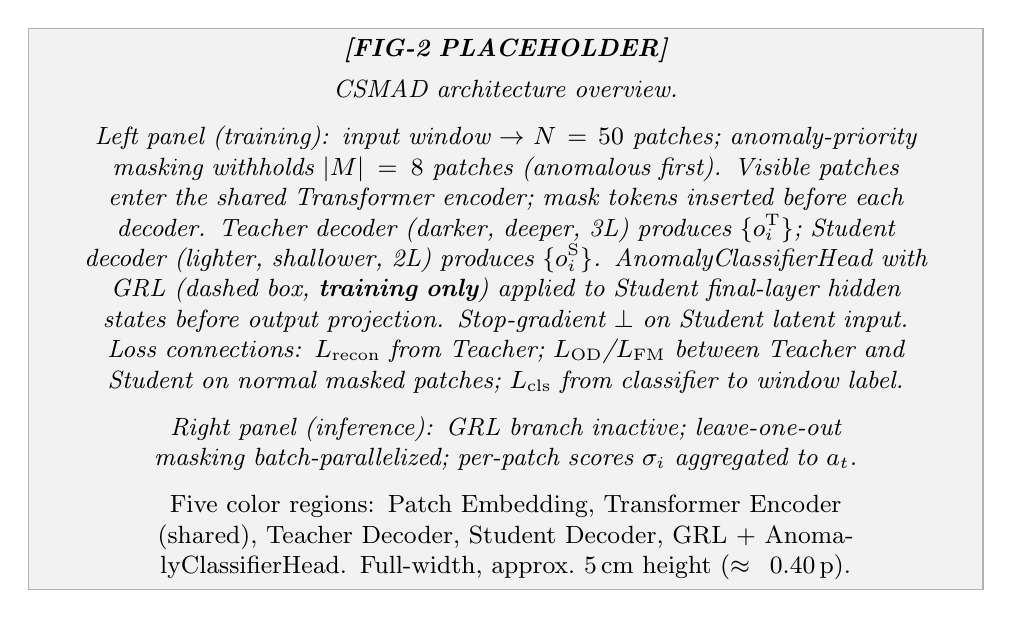
\begin{tikzpicture}
    % height = REGISTRY integrator assumption (5 cm = 0.40p)
    \node[draw=gray!60, fill=gray!10, minimum width=\linewidth, minimum height=5.0cm,
          text width=0.92\linewidth, align=center, font=\small\itshape] (box) {%
      \textbf{[FIG-2 PLACEHOLDER]}\\[4pt]
      CSMAD architecture overview.\\[6pt]
      \textit{Left panel (training):} input window $\to$ $N=50$ patches; anomaly-priority
      masking withholds $|M|=8$ patches (anomalous first). Visible patches enter the shared
      Transformer encoder; mask tokens inserted before each decoder. Teacher decoder (darker,
      deeper, 3L) produces $\{o^{\mathrm{T}}_i\}$; Student decoder (lighter, shallower, 2L)
      produces $\{o^{\mathrm{S}}_i\}$. AnomalyClassifierHead with GRL (dashed box,
      \textbf{training only}) applied to Student final-layer hidden states before output
      projection. Stop-gradient $\perp$ on Student latent input. Loss connections: $L_{\mathrm{recon}}$
      from Teacher; $L_{\mathrm{OD}}$/$L_{\mathrm{FM}}$ between Teacher and Student on normal
      masked patches; $L_{\mathrm{cls}}$ from classifier to window label.\\[6pt]
      \textit{Right panel (inference):} GRL branch inactive; leave-one-out masking
      batch-parallelized; per-patch scores $\sigma_i$ aggregated to $a_t$.\\[6pt]
      \normalfont Five color regions: Patch Embedding, Transformer Encoder (shared), Teacher
      Decoder, Student Decoder, GRL + AnomalyClassifierHead. Full-width, approx.\ 5\,cm
      height ($\approx 0.40$\,p).
    };
  \end{tikzpicture}
  \caption{CSMAD architecture overview.
    \textit{Left panel (training)}: the input window is split into $N$ patches;
    anomaly-priority masking withholds $|M|$ patches (anomalous patches masked first).
    Visible patches enter the shared Transformer encoder; mask tokens are inserted before
    each decoder.
    The Teacher decoder (darker, deeper) produces reconstructions $\{o^{\mathrm{T}}_i\}$;
    the Student decoder (lighter, shallower) produces $\{o^{\mathrm{S}}_i\}$.
    An AnomalyClassifierHead with gradient reversal (dashed box, labeled \textbf{training only})
    is applied to the Student's final-layer hidden states before the output projection.
    Loss connections: $L_{\mathrm{recon}}$ from Teacher outputs; $L_{\mathrm{OD}}$ and
    $L_{\mathrm{FM}}$ between Teacher and Student on normal masked patches; $L_{\mathrm{cls}}$
    from classifier head to window label.
    The encoder receives no gradient from Student or GRL (stop-gradient $\perp$).
    \textit{Right panel (inference)}: GRL branch inactive; leave-one-out masking patterns
    batch-parallelized; per-patch scores $\sigma_i$ averaged to point-level scores $a_t$.}
  \label{fig:architecture}
\end{figure}

CSMAD comprises five functional blocks (Figure~\ref{fig:architecture}): a linear patch
embedding, a shared Transformer encoder, a Teacher decoder, a Student decoder, and a
training-only adversarial branch that couples the Student decoder's hidden states to a
window-level anomaly classifier through gradient reversal.
The encoder receives only the \emph{visible} patches; each decoder reconstructs the full window
from the latent sequence, the Teacher strictly deeper than the Student
(Section~\ref{sec:decoders}).
The Student and GRL branches receive a stop-gradient copy of the encoder output, so the encoder
is optimized exclusively by the Teacher's reconstruction objective.
The adversarial signal therefore cannot corrupt the normal-pattern representation on which the
anomaly score is based.

\subsection{Patch Embedding and Masking}
\label{sec:masking}

\paragraph{Linear patch embedding.}
Each patch $\mathbf{P}_i$ is flattened and projected to a token
$\mathbf{z}_i = \mathbf{E}\,\mathrm{vec}(\mathbf{P}_i) + \mathbf{b} \in \mathbb{R}^{d_{\mathrm{model}}}$,
where $\mathbf{E}$ is a learned linear embedding.
Projecting an entire patch --- $s$ timesteps across all $F$ channels --- into a single token
encodes cross-channel correlations directly in the token, following the linear patchify
principle of MAE~\cite{he2022mae}.

\paragraph{Anomaly-priority masking.}
With masking ratio $\rho$, a fraction $|M| = \mathrm{round}(N \times \rho)$ of the patches is
withheld from the encoder, which processes only the $|V| = N - |M|$ visible tokens.
When patch-level labels are available, each patch receives a priority
$\pi_i = 10^3 \cdot y^p_i + \eta_i$, with $\eta_i \sim \mathrm{Uniform}(0,1)$ breaking ties,
and the $|M|$ highest-priority patches form the masked set: anomalous patches are masked first,
any remaining slots drawn at random from normal patches (formal selection rule in
\ref{sec:aux_formulations}).

Anomaly-priority masking addresses a structural imbalance of contaminated training: anomalous
patches are rare, so stochastic masking seldom selects them, and the model gains little
experience reconstructing anomalous correlation patterns.
It is a training-time mechanism; at test time windows are scored under the deterministic
leave-one-out masking of Section~\ref{sec:scoring}, with no label input.

\subsection{Asymmetric Teacher--Student Decoders}
\label{sec:decoders}

\paragraph{Encoder.}
The visible tokens pass through a Transformer encoder of depth $n_e$ (Pre-Layer-Normalization~\cite{xiong2020prenorm}, multi-head self-attention, GELU), producing latents $\{h^{\mathrm{enc}}_i\}_{i \in V}$.

\paragraph{Teacher decoder.}
Learnable mask tokens are inserted at positions in $M$, position embeddings are added, and the
full sequence is passed through a self-attention-only decoder of depth $n_{\mathrm{T}}$ following
the standard MAE design~\cite{he2022mae}; a linear head projects hidden states
$\{h^{\mathrm{T}}_i\}$ to reconstructions $\{o^{\mathrm{T}}_i\}$.

\paragraph{Student decoder.}
The Student is structurally identical but shallower ($n_{\mathrm{S}} < n_{\mathrm{T}}$), with
separate mask tokens, hidden states $\{h^{\mathrm{S}}_i\}$, and outputs $\{o^{\mathrm{S}}_i\}$;
critically, its input latent carries a stop-gradient,
$h^{\mathrm{S}}_{\mathrm{in},i} = \mathrm{stopgrad}(h^{\mathrm{enc}}_i)$ for $i \in V$.

\paragraph{Why the capacity gap matters.}
A deeper Teacher accurately captures the joint normal correlation structure; the shallower Student
replicates it on recurring normal patterns but fails more severely on the correlation patterns
characteristic of anomalies than a matched-capacity decoder would
(quantified in \ref{sec:extended_ablations}).
Consequently, the output discrepancy carries a stronger anomaly signal than reconstruction error
alone.
This adapts the self-distillation principle of~\cite{zhang2022selfdistill,ristea2024sdmae} to a
contaminated setting where labeled anomalies additionally widen the discrepancy at known fault
locations.

\paragraph{Teacher-only warmup.}
For a fixed initial number of epochs the Student forward pass is skipped and only the Teacher
branch is trained, so the Student begins its adversarial role against a stable
normal-reconstruction reference; we treat this warmup as a training-stability device, not an
independent contribution.

\paragraph{GRL dual-$\lambda$ structure.}
Two independent quantities govern the gradient reversal branch once the Student is active.
The \textbf{loss weight} $\lambda_{\mathrm{GRL}}$ is computed adaptively from the clamped ratio
of main-loss to GRL-loss gradient norms, evaluated per batch and applied as the previous epoch's
average, so the adversarial loss neither dominates nor vanishes.
The \textbf{reversal coefficient} $\lambda_{\mathrm{rev}}$ scales the backward gradient through
the GRL on the sigmoid schedule of Ganin et al.~\cite{ganin2016dann}, growing from ${\approx}0.02$ to
${\approx}1$ over the student-training phase so that suppression strengthens without
destabilizing early Student learning (exact rules in \ref{sec:aux_formulations}).

\subsection{Label-Guided Training}
\label{sec:label_training}

Three loss components couple labeled anomaly information to the model at different levels of the
learning process.

\paragraph{Output discrepancy loss $L_{\mathrm{OD}}$.}
Let $P_n = \{i \in M : y^p_i = 0\}$ be the masked patches labeled normal; $L_{\mathrm{OD}}$
penalizes the discrepancy between the Student's output and the Teacher's detached output on this
subset only:
\begin{equation}
  L_{\mathrm{OD}} = \frac{1}{|P_n| \cdot s \cdot F}
    \sum_{i \in P_n} \left\| o^{\mathrm{T}}_i - o^{\mathrm{S}}_i \right\|^2
  \label{eq:lod}
\end{equation}
Anomalous patches are excluded from $L_{\mathrm{OD}}$: the Student is steered to agree with
the Teacher on normal patterns while remaining free to deviate at anomaly locations.

\paragraph{Feature matching loss $L_{\mathrm{FM}}$.}
A hidden-space regularizer penalizes Teacher--Student representation distance on normal masked
patches ($h^{\mathrm{T}}_i$ detached):
\begin{equation}
  L_{\mathrm{FM}} = \frac{1}{|P_n| \cdot d_{\mathrm{model}}}
    \sum_{i \in P_n} \left\| h^{\mathrm{T}}_i - h^{\mathrm{S}}_i \right\|^2
  \label{eq:lfm}
\end{equation}
This prevents the Student from satisfying the output-level constraint without tracking the
Teacher's internal structure; $\lambda_{\mathrm{FM}}$ follows the same adaptive mechanism as
$\lambda_{\mathrm{GRL}}$, and the term is a training-only regularizer absent from the inference
score.

\paragraph{GRL anomaly suppression loss $L_{\mathrm{cls}}$.}
Whereas SDMAE suppresses anomaly reconstruction in the target/loss space (training the model to
reconstruct anomaly-free targets~\cite{ristea2024sdmae}), our GRL operates in the gradient space
of the Student's internal representation.
A two-layer MLP head $g_\phi$ takes as input the Student hidden state of each masked patch and
predicts whether the enclosing window contains an anomaly ($y^w$ broadcast to all masked patches;
strictly, the target indicates an anomaly within the masked region, which coincides with $y^w$
under anomaly-priority masking).
The head is trained with a focal-style binary cross-entropy (BCE) variant for severe class
imbalance: unlike the standard focal loss~\cite{lin2017focal}, whose modulating factor derives
from the raw prediction, the modulating factor here derives from the class-prior-weighted
cross-entropy itself (exact form: Eq.~\ref{eq:lcls_app}).
The gradient reversal layer~\cite{ganin2016dann} between head and Student hidden states is an
identity map in the forward pass and multiplies the gradient by $-\lambda_{\mathrm{rev}}$ in the
backward pass; the resulting adversarial gradient, proportional to
$-\lambda_{\mathrm{rev}} \cdot \lambda_{\mathrm{GRL}}$, penalizes anomaly-discriminative
information in the Student's hidden states, pushing the Student toward anomaly-\emph{invariant}
internal states.

\paragraph{Why gradient reversal is necessary beyond loss bifurcation.}
Excluding anomalous patches from $L_{\mathrm{OD}}$ removes the requirement that the Student
match the Teacher's output at those locations, but it does not actively remove anomaly information
from the Student's representation.
Although anomalous patches are preferentially masked and therefore hidden from the encoder, the
visible patches of an anomalous window still carry the surrounding anomalous context, and the
shared encoder embeds that context into the latent sequence that both decoders read.
Over repeated exposure to labeled anomalies during training, the Student can learn to exploit
this contextual signal to reconstruct anomalous patterns, thereby reducing the discrepancy where
it is most diagnostic.
Gradient reversal closes this route at the representational level: the adversarial gradient
suppresses anomaly-discriminative information in the Student's hidden states regardless of what
supervision enters through the loss.

\paragraph{Total training loss.}
\begin{equation}
  L_{\mathrm{total}} = L_{\mathrm{recon}} + L_{\mathrm{OD}}
    + \lambda_{\mathrm{FM}} \cdot L_{\mathrm{FM}}
    + \lambda_{\mathrm{GRL}} \cdot L_{\mathrm{cls}}
  \label{eq:ltotal}
\end{equation}
where $L_{\mathrm{recon}}$ is the Teacher's mean squared reconstruction error on masked
positions; the GRL term contributes only when the batch contains a positive window.

\subsection{Anomaly Scoring and Inference}
\label{sec:scoring}

\paragraph{Leave-one-out masking.}
Each test window is scored under $N$ masking patterns --- each masking a single patch in
isolation, with all $N$ masked variants processed as one batched forward pass --- eliminating
cross-patch interference at an inference cost of approximately $N$ single-window forward passes;
this cost is an acknowledged limitation.

\paragraph{Patch-level anomaly score.}
For each masked patch $i$, the Teacher reconstruction error $r_i$ (MSE over its $s \cdot F$
values) and the Teacher--Student discrepancy
$d_i = \|o^{\mathrm{T}}_i - o^{\mathrm{S}}_i\|^2 / (s \cdot F)$ are computed; the GRL
classifier is not used at inference.
The discrepancy is adaptively scaled to the magnitude of $r_i$,
\begin{equation}
  \tilde{d}_i = d_i \cdot \frac{\bar{r} + \varepsilon}{\bar{d} + \varepsilon},
  \quad \varepsilon = 10^{-4}
  \label{eq:dscale}
\end{equation}
Here, $\bar{r}$ and $\bar{d}$ are the means of the patch-level reconstruction errors and
discrepancies, respectively, over all (window, patch) pairs of the evaluated series, computed
once per entity.
The two components are then combined at a fixed ratio:
\begin{equation}
  \sigma_i = r_i + \frac{\tilde{d}_i}{c}, \quad c = 4
  \label{eq:sigma}
\end{equation}
Adaptive scaling prevents either component from dominating by sheer magnitude, which varies
substantially across datasets; $c$ sets the discrepancy contribution to one quarter of the
reconstruction term after scaling.

\paragraph{Point-level aggregation.}
Each timestep $t$ belongs to one or more (window, patch) pairs, where $u$ indexes the covering
windows, and its final score is the mean of $\sigma_i$ over all such pairs:
\begin{equation}
  a_t = \frac{\displaystyle\sum_{(u,i):\; t \in \mathbf{P}^u_i} \sigma^u_i}
             {\left|\{(u,i):\; t \in \mathbf{P}^u_i\}\right|}
  \label{eq:agg}
\end{equation}
Averaging across overlapping windows provides an ensemble effect that reduces
context-dependent reconstruction variance.

%% PDF QA r1 MAJOR-8: keep this section's floats from drifting past the section end
\BodyFloatBarrier
